\clearpage

\def\chaptertitle{Performance Evaluation}

\lhead{\emph{\chaptertitle}}

\chapter{\chaptertitle}
\label{ch:performance-evaluation}

In this chapter, we begin by discussing the underlying hardware configuration, and assumptions made before beginning the auto-scaling experiments in section \ref{sec:ch5-hardware-assumptions}. The cluster configuration, which involves the resource divisions between servers, overall cluster architecture, and deployment resources is discussed in section \ref{sec:ch5-cluster-config}.

\section{Assumptions and Underlying Hardware}
\label{sec:ch5-hardware-assumptions}

For the hardware setup, servers in the Melbourne Research Cloud \footnote{\url{https://docs.cloud.unimelb.edu.au/}} were leveraged to deploy microservices on. The set up consisted of 6 servers, using a total of 16 CPU cores and 48GB of memory. These servers were separated into a cloud and edge layer. The servers on the cloud layer have a significantly higher amount of CPU cores and memory assigned compared to the servers in the edge layer, to simulate the scarcity of resources in the edge layer. Furthermore, a simulated latency was added between inter-layer server communication to mimic the perceived distance between edge nodes and large data-centres.\par

Each server consists of an Ubuntu 22.04 operating system. Kubernetes v1.28.2 is used as the container orchestration technology behind the experimental micro service setup. For maximum flexibility, a bare-metal implementation of Kubernetes is used, instead of ready made solutions available from Amazon or Google. The control plane is deployed on the cloud layer, while the data plane is on the edge layer. Furthermore, several assumptions were made before proceeding with the experimentation:

\begin{itemize}
    \item The only auto-scaling performed would be horizontal pod auto-scaling. Vertical and cluster auto-scaling were out of scope of the project.
    \item The pods on which auto-scaling are not applied will have the maximum possible resource allocation to remove the chances of bottleneck.
    \item At no point in the experiment would a node be taken down, or new node be added.
    \item The autoscaler assumes that every node in the edge layer is an equally likely candidate for scheduling pods on.
\end{itemize}

\section{Cluster Configuration}
\label{sec:ch5-cluster-config}

The hardware was divided into the cloud and edge layer as depicted in table \ref{tab:cluster-hw-overview}. The control plane was divided into two servers, one for handling the Kubernetes control plane scheduling, API service, and etcd deployments, and the other for storing the Prometheus database, along with the microservice Jaeger metrics collection. The edge layer consisted of four servers with far less resources, to depict the difference in computing power. The network layer between the edge and cloud deployments also contained a simulated latency to denote the perceived geographical distance between them.\par

%TC:ignore
\begin{table}
    \caption{Cluster architectural layout}\label{tab:cluster-hw-overview}
    \centering
    \begin{tabular}{|l|l|l|l|}
        \hline
        Node & Layer & CPU (cores) & Memory (GB)\\
        \hline
        Control-Plane-K8s & Cloud & 4 & 16\\
        Control-Plane-DB  & Cloud & 4 & 16\\
        Data-Plane-1      & Edge  & 2 & 4\\
        Data-Plane-2      & Edge  & 2 & 4\\
        Data-Plane-3      & Edge  & 2 & 4\\
        Data-Plane-4      & Edge  & 2 & 4\\
        \hline
    \end{tabular}
\end{table}
%TC:endignore

The cloud and edge nodes were differentiated in through Kubernetes through the internal labelling system. A key ``type'' with value either ``cloud'' or ``edge'' was added to each node. This would enable the scheduler to automatically consider restricting the deployment of pods to particular nodes. For example, the Prometheus deployment would only be deployed on the node of type cloud. This process is known as ``node affinity'' \cite{santos2019towards}.\par

There were several options to deploy the social media application to Kubernetes. Manually cloning them from the repository, creating the custom resource definitions (CRDs), and deploying the YAML files is an option which gives maximum flexibility, but is difficult to debug if things go wrong. Due to this, the Kubernetes package manager Helm was used. Helm \footnote{\url{https://helm.sh/}} is another open-source project whose primary goal involved streamlining the installation, maintenance, and removal of Kubernetes deployments. This is achieved through the use of a Helm chart, which details the configuration of the project, and how to update and access it.\par

Therefore the social media application was the first to be deployed on Kubernetes. However, before deploying the application, the primary deployments to be tested needed to be configured. Based on the ``wrk2'' benchmark that was discussed above, two APIs were identified. One was a GET call to the user's home timeline, and the other was a POST method made by the user to create a post.\par

First, a default social media deployment was installed using the helm command below:

\begin{lstlisting}[
  caption={Social network installation using Helm},
  captionpos=t,
  label={lst:social-network-helm-install},
  language=bash
]
$ helm install social-media \
/DeathStarBench/socialNetwork/helm-chart/Chart.yaml -n default
\end{lstlisting}

With the social media network now deployed, a workload for both GET and POST commands were invoked to generate the latency trace on Jaeger, as depicted in listing \ref{lst:wrk2-api-calls}.

\begin{lstlisting}[
  caption={Social network installation using Helm},
  captionpos=t,
  label={lst:wrk2-api-calls},
  float=ht,
  language=bash
]
$ WRK2="/DeathStarBench/wrk2/wrk -D exp -t 1 -c 1 -d 1 -L -s -R 1"
$ HT=./wrk2/scripts/social-network/read-home-timeline.lua
$ CS=./wrk2/scripts/social-network/compose-post.lua
$ IP=$(kubectl get svc nginx-thrift --template '{{.spec.clusterIP}}')
$ PORT=8080
$ $WRK2 $HT http://$IP:$PORT/wrk2-api/home-timeline/read
$ $WRK2 $HT http://$IP:$PORT/wrk2-api/post/compose
\end{lstlisting}

With the traces generated, the deployments which require autoscaling could be identified for each. From the Jaeger traces generated in figure \ref{fig:ht-cp-trace}, it is clear that the two deployments highlighted in purple, namely ``home-timeline-service'', and ``compose-post-service'', were the major bottlenecks in API processing, and thus required autoscaling. Therefore, the helm deployment was updated to assign resources to them. The resources were assigned in a realistic manner consistent with edge deployments, and based on the number of components each deployment answered to. Listing \ref{lst:deploy-resource-update} shows the CPU resources assigned to both deployments.\par

\begin{figure}[htb]
    \centering
    \caption{Home Timeline and Compose Post API trace}
    \label{fig:ht-cp-trace}
    \begin{minipage}{0.25\linewidth}
        %\caption{Home Timeline API trace}
        %\label{fig:home-timeline-trace}
        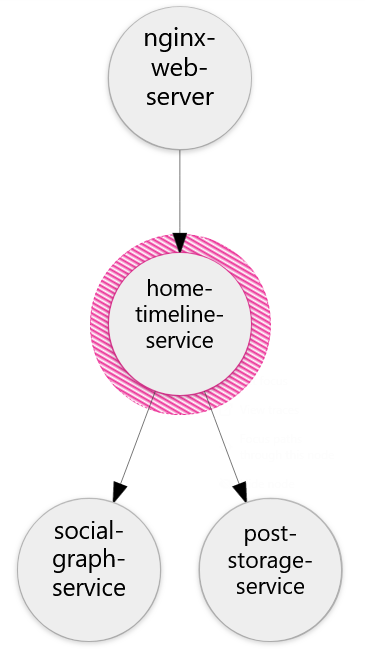
\includegraphics[width=1.0\linewidth]{Figures/Home-Timeline-GET-Trace.png}
    \end{minipage}\hfill
    \begin{minipage}{0.75\linewidth}
        %\caption{Compose Post API trace}
        %\label{fig:compose-post-trace}
        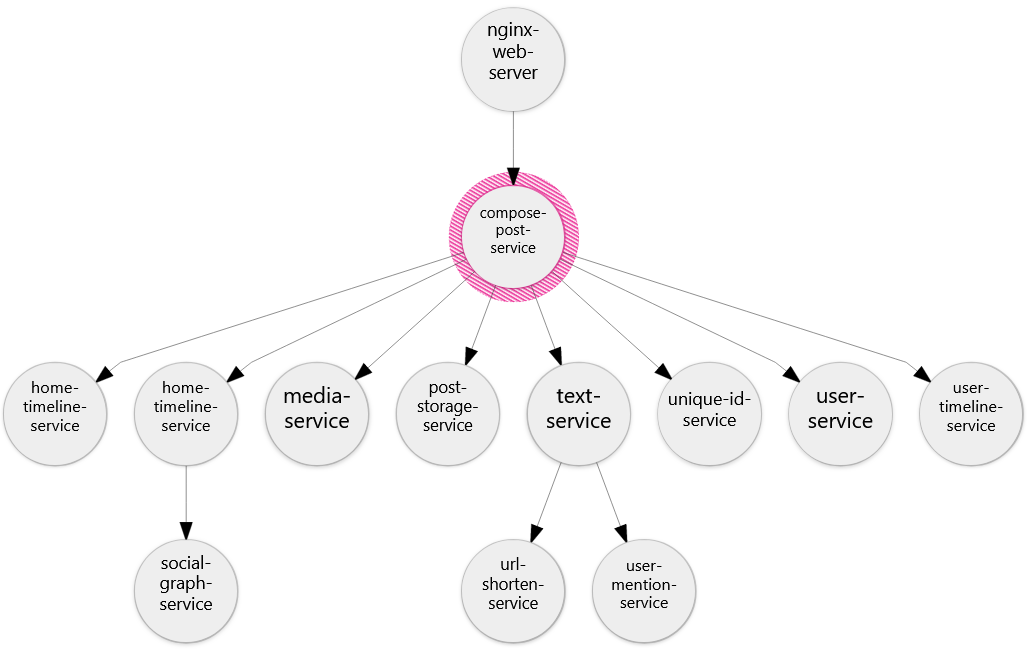
\includegraphics[width=1.0\linewidth]{Figures/Compose-Post-POST-Trace.png}
    \end{minipage}
\end{figure}

\begin{lstlisting}[
  caption={Update resources for bottlenecked deployments},
  captionpos=t,
  label={lst:deploy-resource-update},
  language=bash
]
$ helm upgrade social-media \
/DeathStarBench/socialNetwork/helm-chart/Chart.yaml -n default \
--set-string compose-post-service.container.resources="requests: 
      cpu: "30m"
    limits:
      cpu: "30m"" \
--set-string home-timeline-service.container.resources="requests: 
      cpu: "15m"
    limits:
      cpu: "15m""
\end{lstlisting}

\section{Experiment Setup}
\label{sec:ch5-exp-setup}

Two independent experiments were conducted to verify the performance of the hybrid autoscaler. The social media application was first tested using the GET API to autoscale the home-timeline-service deployment. Then, a more demanding as well as challenging workload was applied to the POST API for autoscaling the compose-post-service deployment. For both these experiments, the workload generation algorithm was used to create realistic daily workloads and tested over the period of one week. Both experiments would configure a flexible SLA latency agreement to be maintained. For the first experiment, the SLA constraint was set to a 150 milliseconds latency, and for the second experiment, it was 1000 milliseconds. The flexible SLA constraint was the primary focus of the experiment, however a moderate and strict SLA constraint was also chosen and tested. The SLA values are shown in table \ref{tab:experiment-sla-values}.\par

%TC:ignore
\begin{table}
    \caption{Experimental SLA constraints}\label{tab:experiment-sla-values}
    \centering
    \begin{tabular}{|l|l|l|}
        \hline
        SLA Type & GET API constraint (ms) & POST API constraint (ms)\\
        \hline
        Flexible    & 150   & 1000\\
        Moderate    & 125   & 900\\
        Strict      & 100   & 800\\
        \hline
    \end{tabular}
\end{table}
%TC:endignore

For the proposed hybrid algorithm to achieve these autoscaling goals within the SLA constraints, the autoscaling subsystems were configured as follows. The reactive autoscaler would check if the CPU utilization of the deployment was exceeding the 50\% threshold. If so, it would scale up based on the cooldowns and tolerations set. The proactive autoscaler on the other hand would check if the forecasted CPU utilization in the next 20 minutes was going to breach the 50\% threshold, and if so, would autoscale with the same configured parameters as the reactive one. The daemon would store the total CPU utilization of the deployment as a time-series for a maximum of seven days, and constantly check for SLA violations to tweak the hyper-parameters of the forecaster as discussed above in section \ref{subsec:ch4-auto-daemon-subsection}. To measure the effectiveness of the hybrid autoscaler, three baseline algorithms were chosen for comparison. All three would autoscale at the CPU threshold of 50\%. Furthermore, these algorithms would be implementations based on the ones discussed in section \ref{sec:ch2-lit-review}.\par

The first was the default Kubernetes horizontal pod autoscaler. No modifications to the configuration were made, thus the scale up cooldown was 0 seconds, while the scale down was 300 seconds. Additionally, the autoscaler had no knowledge of the workload distribution or SLA violations on the edge nodes.\par

The second baseline was an implementation of the reactive traffic aware horizontal pod autoscaler created by Phan et al. \cite{phan2022traffic}. This autoscaler scheduler would compute the ratio of workloads being exerted on the different edge nodes with the deployment pods. Once it did so, it would scale these resources in a commensurate proportion.\par

Finally, the last baseline implementation was the Proactive Pod Autoscaler (PPA) devised by Ju et al. \cite{ju2021proactive}. This algorithm was an open-ended implementation which enabled the user to plugin a deep learning model of their choice. The PPA architecture consisted of three sub-sections, the formulator, evaluator, and updater. An LSTM model was injected into the autoscaler as the model file. This LSTM implementation was similar to the one used in the hybrid autoscaler, however it differed in two key elements. First, the LSTM did not expect pre-processed data without noise, and thus dealt with more complex time-series data. Secondly, due to this additional computation, the LSTM contained a deeper architecture layer with more neural network units. This was required as the algorithm had to correctly predict the complete future workload since there was no reactive autoscaler to fall back on. Over a fixed interval, the algorithm continuously looped through the time-series data and saved the forecast result to a metrics file. The evaluator took these outputs from the metrics file, along with the LSTM from the model file to predict the number of pods to assign in advance, and requested the Kubernetes scheduler for scaling through the API Service. A second loop, known as the update loop, then updated the LSTM model using the latest forecast, and cleared the metrics file. The hyper-parameters were carefully tuned to ensure that the model did not under-perform too significantly. Finally, the PPA architecture did not take into account SLA compliance, and thus SLA metrics were not provided as a feedback for hyper-parameter tuning.\par


\section{Experiment I - GET API Workload}
\label{sec:ch5-exp1-get-api}

In the first experiment, the IoT workload generation algorithm was configured to create a workload aimed at mimicking GET requests. By doing so, the $home-timeline-service$ deployment becomes the bottleneck receiving all of the requests, and thus can be tested using the proposed hybrid autoscaler, as well as the three baseline algorithms. As shown above, the autoscaling threshold was set to 50\% total CPU utilization, and the SLA latency threshold was set to 150 milliseconds.\par

\begin{figure}[htb]
    \centering
    \caption{Experiment I - Total CPU utilization}
    \label{fig:exp1-workload}
    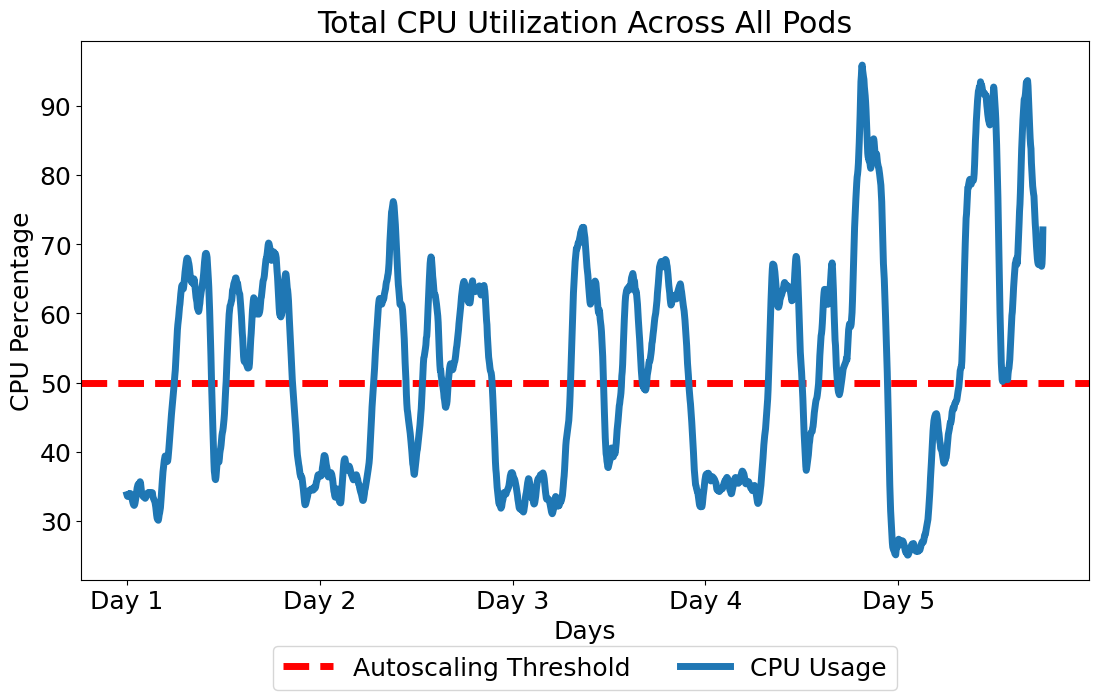
\includegraphics[width=0.6\linewidth]{Figures/GET-Total-CPU.png}
\end{figure}

Figure \ref{fig-exp1-workload} shows the total CPU workload that was generated by algorithm \ref{alg:work-gen} on the $home-timeline-service$ deployment. The data was generated for a total of five days. Each day approximately $510000$ requests were sent to the edge deployment. The daily peak remains at approximately the same percentage, but then increases significantly in the last two days. This can be a depiction of how social network requests may look on the weekends. The total CPU utilization never exceeded 95\% of the total allocated resources shown in listing \ref{lst:deploy-resource-update}. This is expected of a GET request, as while the deployment has to open a connection to the sub-deployments to receive the response, a GET request is typically a database SELECT statement, which takes a comparatively less amount of time as opposed to other operations. This means that the deployment can quickly receive the response from its child components, send the response up to the requester, and then close the connection. Once the connection is closed, all the resources associated with it are freed. Because this operation is so quick, multiple concurrent connections are typically not open, and thus the CPU utilization is not significant.\par

\subsection {Default Kubernetes Autoscaler Baseline}
\label{subsec:ch5-exp1-default-algo}

\begin{figure}[htb]
    \centering
    \caption{Experiment I - Kubernetes Default Autoscaler Latency}
    \label{fig:exp1-default-k8s}
    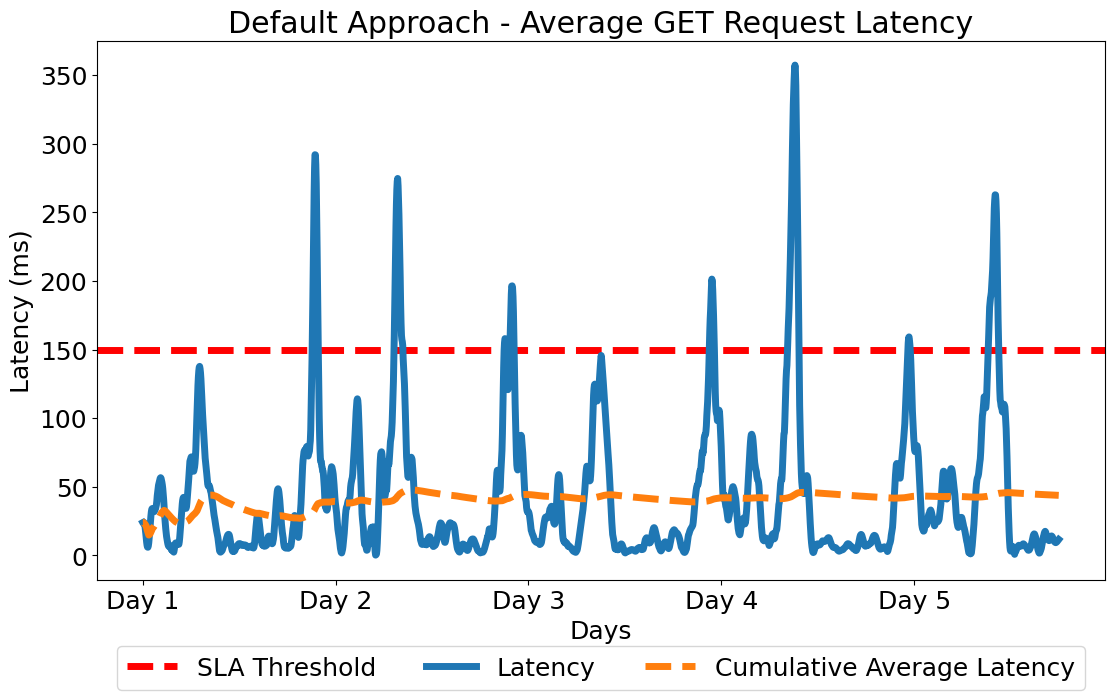
\includegraphics[width=0.6\linewidth]{Figures/Home-Timeline-Default-Latency.png}
\end{figure}

Even with such a workload, a near 100\% CPU utilization on a solitary deployment pod would lead to significant delays. This can be seen when using the default Kubernetes Horizontal Pod Autoscaler, as depicted in figure \ref{fig:exp1-default-k8s}. The autoscaler is merely a primitive reactive implementation with no knowledge of which edge nodes are experiencing heavy traffic, and which ones are not. Thus, it blindly assigns pods to the nodes in a round-robin manner. Additionally, the autoscaler requires a lot of time to register the new pods to the Kubernetes control plane, thus falling victim to the cold start problem. This results in significant latency spikes before the resources are adjusted. In the figure, it can be seen that the latency exceeds 300 milliseconds at some points, which would render the edge deployment unusable. Additionally, by the end of the fifth day of testing, the average latency of the social-network was nearly 50 milliseconds. Through this experiment, it can be concluded that the default Kubernetes autoscaler is completely unsuitable for edge auto-scaling use-cases which are SLA sensitive.\par

\subsection {Reactive THPA Autoscaler Baseline}
\label{subsec:ch5-exp1-reactive-algo}

\begin{figure}[htb]
    \centering
    \caption{Experiment I - THPA Reactive Autoscaler Latency}
    \label{fig:exp1-reactive-k8s}
    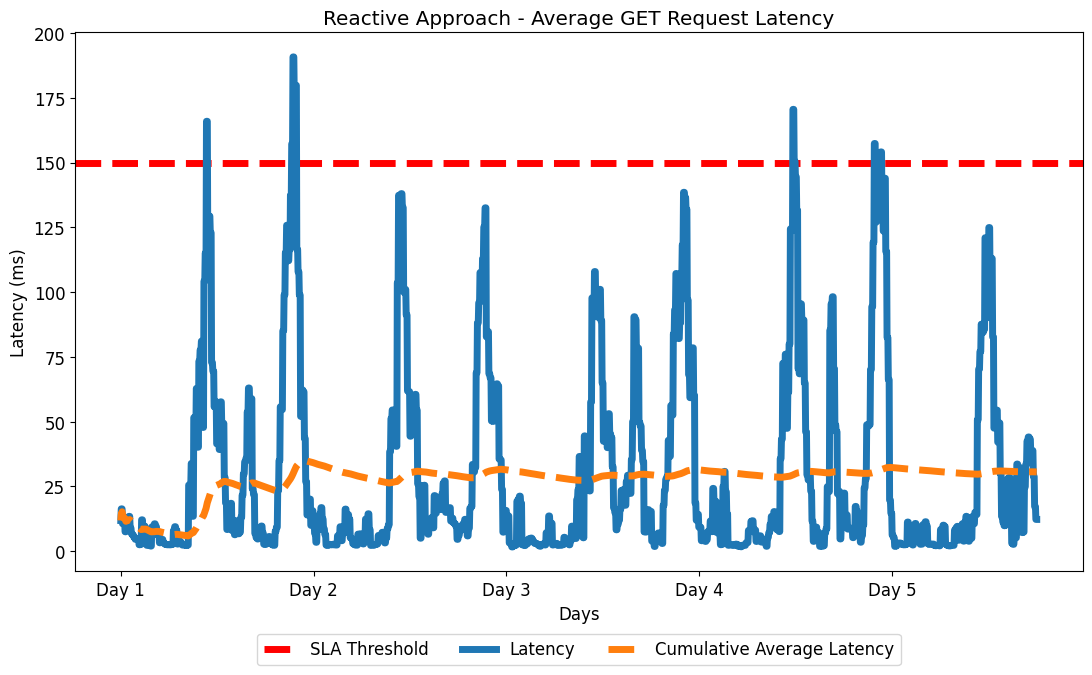
\includegraphics[width=0.6\linewidth]{Figures/Home-Timeline-Reactive-Latency.png}
\end{figure}

The second autoscaling baseline solution to be tested was an in-house implementation of the reactive traffic aware horizontal pod autoscaler solution by Phan et al. \cite{phan2022traffic}. Unlike the default Kubernetes autoscaler, THPA keeps track of which edge node was receiving significant number of requests and assigns pods to the nodes accordingly. This strategy results in a significantly improved latency graph, as can be seen in Figure \ref{fig:exp1-reactive-k8s}. While the algorithm still suffers from the cold start problem, the more intelligent assignment of resources results in less availability issues, ensuring that the latency spikes which are seen are not as drastic as the ones in the default implementation. However, due to the cold start problem, the SLA threshold of 150ms is still regularly breached, resulting in several violations and loss of availability. However these breaches never exceed the 200ms mark, and thus complete loss of system availability is never seen. Furthermore, the average latency over the experimental time frame was lower than what was seen in the default implementation, hovering at around 25-30 milliseconds. Therefore, the reactive approach, while a valid solution for most edge solutions, is not adequate for an SLA-constrained architecture, and further modifications are required.\par

\subsection {Proactive PPA Autoscaler Baseline}
\label{subsec:ch5-exp1-proactive-algo}

The final baseline algorithm to be deployed for auto-scaling $home-timeline-service$ was an implementation of the proactive pod autoscaler (PPA) based on Ju et al. \cite{ju2021proactive}. Unlike the previous two baseline algorithms, this one attempts to predict the workload before it is requested, thus eliminating the cold start issue. In ideal conditions, this would result in the SLA threshold not being violated, and it being a viable solution for edge paradigms. However, experimental results showed otherwise.\par

\begin{figure}[htb]
    \centering
    \caption{Experiment I - PPA Proactive Autoscaler Latency}
    \label{fig:exp1-proactive-k8s}
    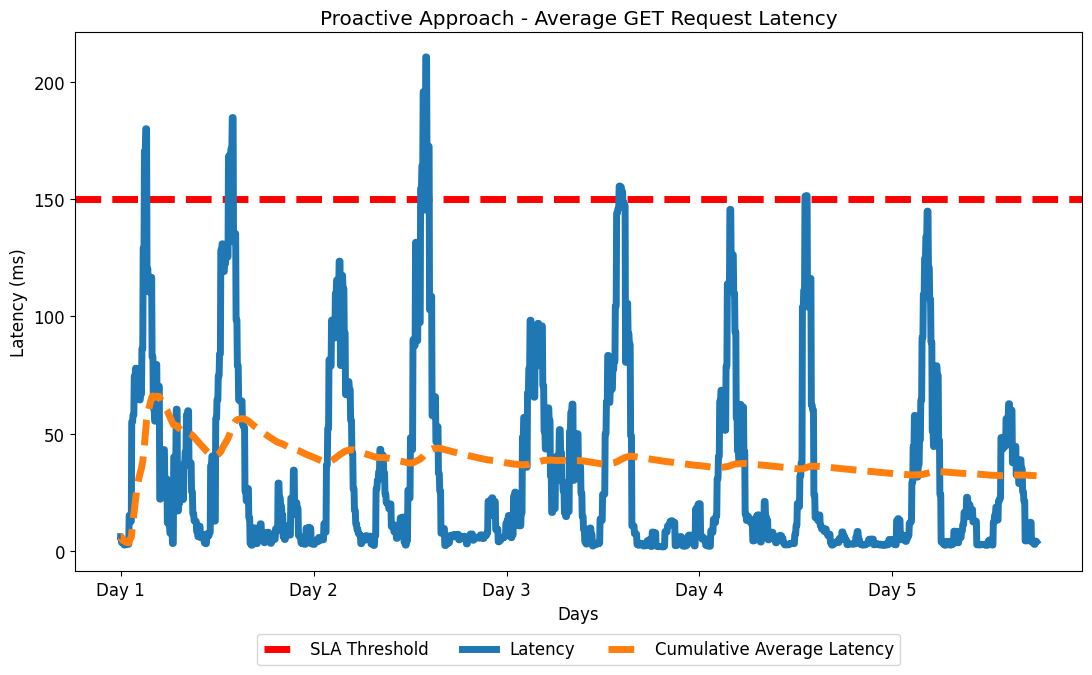
\includegraphics[width=0.6\linewidth]{Figures/Home-Timeline-Proactive-Latency.png}
\end{figure}

Because the autoscaler is purely proactive, it must be a deep LSTM model with several layers and large training epochs. This deep model takes more than 20 minutes to properly train and validate for it to predict 24 hours of data, similar to what our proposed hybrid solution predicts. This is due to the edge architectures lack of resources and storage compared to the cloud layer. Figure \ref{fig:exp1-proactive-k8s} shows this in action. Initially it is observed that the latency continually spikes, causing a large amount of SLA violations, more than what the reactive autoscaler caused. However, after a few days of training, the rolling update structure of the LSTM weights took over, reducing the training time by taking advantage of the early stopping callback in the LSTM model, and managing to stabilize the latency. However, this affect does not always manage to stem the latency overflow, as is shown when the same algorithm was tested using the POST API in section \ref{subsec:ch5-exp2-post-api}.

While the SLA violations were not as severe as the ones seen in the Default autoscaler baseline, they were comparatively greater than the reactive approach, with the latency exceeding 200 milliseconds for several minutes during the day, causing a loss of availability. The average latency was almost as large as what was seen in the default autoscaler baseline, approaching 50 milliseconds due to the issues inherent in attempting to forecast the entire time-series data curve.  Due to these issues, the algorithm itself was demonstrated as unsuitable for SLA-constrained paradigms.\par

\subsection {Proposed Hybrid Autoscaler}
\label{subsec:ch5-exp1-hybrid-algo}

\begin{figure}[htb]
    \centering
    \caption{Experiment I - Hybrid Autoscaler Latency}
    \label{fig:exp1-hybrid-k8s}
    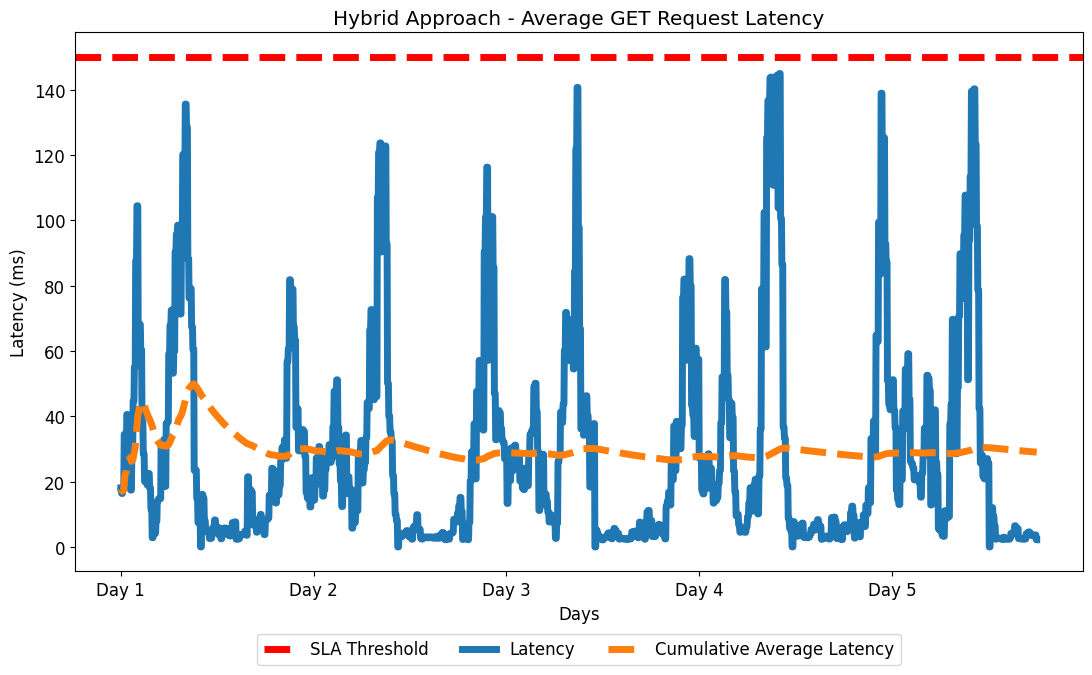
\includegraphics[width=0.6\linewidth]{Figures/Home-Timeline-Hybrid-Latency.png}
\end{figure}

Finally, with the baselines being established in a default, reactive, and proactive approach, the hybrid algorithm was tested on the five days of generated workload. This approach demonstrated how it could mitigate the issues seen in both reactive and proactive auto-scaling approaches. The autoscaler was extremely lightweight, and easy to configure, since there was no hyper-parameter tuning required. Building on top of this light weight, the proactive forecaster was able to forecast the beginning of the workload spike accurately, thus leading to it eliminating the issue of cold start. The forecaster could not accurately predict the middle and end of the daily workloads, however this was not an issue, since the reactive algorithm was capable of taking over the auto-scaling process, and maintaining the necessary resources to avoid SLA violations. Figure \ref{fig:exp1-hybrid-k8s} shows the complete latency graph for the hybrid experiment.\par

From the graph, it is clear that for the GET request experiment, no SLA violations were present for the duration of the five day workload. Thus in this case, the autoscaler daemon did not require to kick in and modify the hyper-parameters of the forecaster. The average latency experienced by the social network is also comparatively low, achieving results similar to the THPA reactive implementation with the value hovering at around 30 milliseconds. This performance is a significant improvement over the baseline algorithms, and demonstrated the efficacy of such a model in an edge architecture deployment.\par


\subsection {CPU Workload Distribution Per Autoscaler}
\label{subsec:ch5-exp1-workload-dist}

The distribution of CPU workload across the deployment pods was another important metric to factor in to the analysis. With an autoscaler threshold being set at $\mathcal{A}$, ideally the distributed workload should hover at $\frac{\mathcal{A}}{2}$. When this workload distribution value $workload \rightarrow \mathcal{A}$ such that the total CPU workload being exerted on each pod is not putting a burden on the social network, driving up latency. On the other hand, when $workload \rightarrow \mathcal{0}$, the returns when it comes to latency reduction are extremely low, while the number of resource pods being assigned to the deployment undergoing auto-scaling are increasing significantly. This in turn increases the cost of running the underlying edge architecture, making this autoscaler an unprofitable alternative.\par

\begin{figure}[htb]
    \centering
    \caption{Experiment I - Autoscaler CPU Workload Distribution Comparison}
    \label{fig:exp1-cpu-avg-dist}
    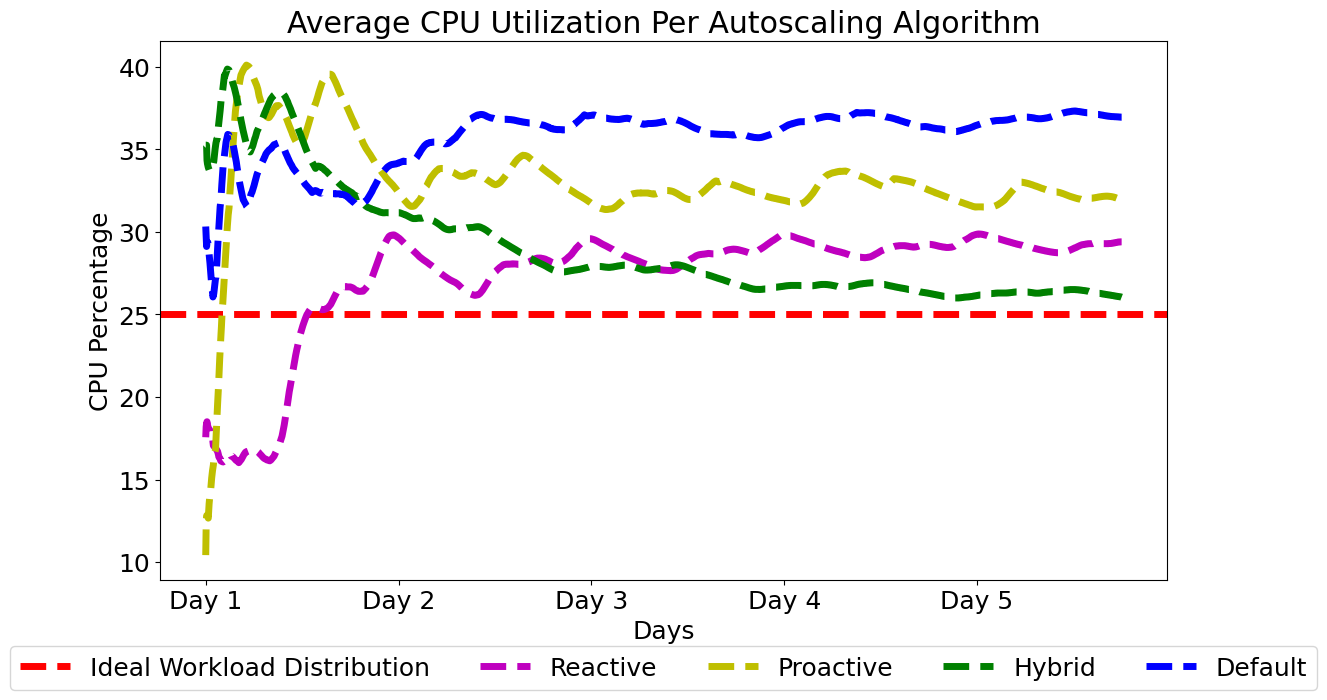
\includegraphics[width=0.6\linewidth]{Figures/Home-Timeline-CPU-Usage.png}
\end{figure}

Figure \ref{fig:exp1-cpu-avg-dist} shows the average CPU utilization of all the deployment pods for the three baseline algorithms, and the proposed hybrid solution. As expected, the default Kubernetes horizontal pod autoscaler performs the worst, with the average utilization hovering around 35\%. The proactive forecaster has a utilization of approximately 33\%, with it being held back by the forecaster complexity and resource intensive training. The reactive approach was the most lightweight autoscaler, and thus performed well with the CPU utilization of around 30\%. Finally, the hybrid autoscaler performed the best of the four compared algorithms, with the utilization of approximately 26\%. This demonstrates that, while the hybrid approach is able to mitigate or eliminate SLA violations, it does so in a manner which is both using a lightweight deployment, and with an algorithm which does not deploy resources in a wasteful manner.\par

\subsection{SLA Violations Analysis}
\label{subsec:ch5-exp1-sla-violations}

As demonstrated above, the hybrid autoscaler performed significantly better than the baseline approaches. However, this was only compared using the flexible SLA thresholds. As a reminder, this was the most lenient threshold possible. For a more thorough demonstration, the algorithms needed to be tested on other thresholds.\par

To achieve this, all four algorithms were tested again on the moderate and strict SLA violation thresholds for the GET API, as displayed in table \ref{tab:experiment-sla-values}. The IoT workload generation algorithm was once again used to generate this, however this time the workload was run for two days. This was done to get the SLA violation percentage for approximately 1.02 million GET requests.\par

\begin{figure}[htb]
    \centering
    \caption{SLA Violation Percentage For GET API Thresholds}
    \label{fig:exp1-sla-violation-bar}
    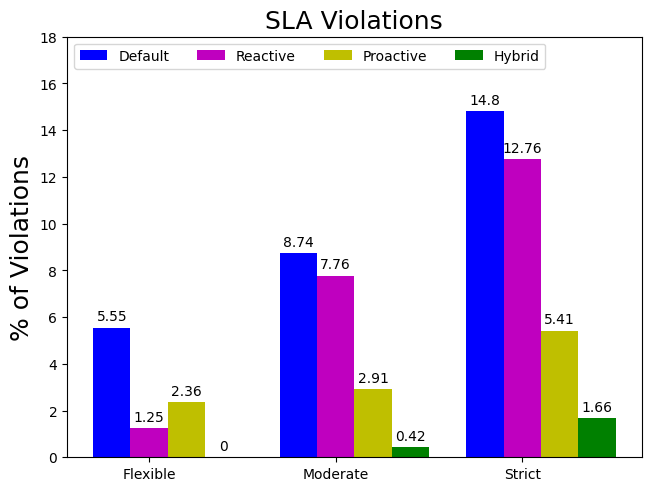
\includegraphics[width=0.6\linewidth]{Figures/Home-Timeline-SLA-Violations.png}
\end{figure}

Figure \ref{fig:exp1-sla-violation-bar} shows the SLA violations for the three different categories. The flexible percentages are taken from the data taken from the five day experiment using the 150 millisecond threshold. The default Kubernetes autoscaler performed the worst, with 5.55\% of all requests being above the SLA threshold. The proactive PPA algorithm came next with a violation rate of 2.36\%, with the amount of violations being increased due to the complexity of the training model. The reactive THPA algorithm performed well, the low resource deployment, combined with the low overhead of GET requests ensured that it only violated the SLA thresholds of 1.25\% of requests. Finally, as seen above, the hybrid autoscaler performed the best of the four implementations, being able to serve all the requests with a 0\% SLA violation rate. This would qualify the hybrid architecture for a ``highly available'' SLA deployment.\par

While the flexible SLA threshold showed impressive results for three out of the four algorithms, the moderate threshold of 125 milliseconds was a more difficult constraint to maintain. The importance of the cold start problem when it comes to SLA latency was exposed in this threshold, as the default Kubernetes implementation and the reactive THPA autoscaler showed extremely similar results, violating 8.74\% and 7.76\% of requests respectively. On the contrary, the proactive PPA approach was able to demonstrate how even mitigating the cold start problem while not being able to eliminate it completely can still have benefits, with the algorithm violating just 2.91\% of requests. Finally, the hybrid autoscaler still achieved the best results. There were violations at the beginning of the experiment, resulting in 0.42\% of requests being above the SLA threshold. However, this was quickly counteracted by the autoscaler daemon, which modified the hyper-parameters to stabilize the latency. Once this was achieved, the hyper-parameters were dropped back down to the default values, and the autoscaling continued as normal.\par

Finally, the strict SLA threshold of 100 milliseconds was tested, which proved extremely difficult to comply with. Once again, the default and reactive autoscalers performed similarly poorly, with 14.8\% and 12.76\% of requests not meeting the SLA threshold respectively. The proactive algorithm distinguished itself from the reactive ones, clearly showing the importance of the cold start problem, by only violating 5.41\% of the requests. However, in this scenario as well, the hybrid algorithm performed significantly better with only 1.66\% of violations. Even though the algorithm would occasionally violate the threshold, the combined approach, along with the daemon's heuristic feedback was able to control the violation rate far better than the three baseline approaches.\par

In conclusion, the hybrid approach proved to be the best autoscaler when it came to an edge deployment with minimal resources available. Furthermore, the algorithm was adaptable, able to display considerably improved performance in comparison with other reactive and proactive approaches using different SLA thresholds. It was able to achieve this with minimal parameter configurations required by the user. The total number of requests, along with the number of violations is provided in the table \ref{tab:sla-violation-count}.

%TC:ignore
\begin{table}
    \caption{SLA Violation Counts For The Autoscalers}\label{tab:sla-violation-count}
    \centering
    \begin{tabular}{|l|l|l|l|l|}
        \hline
        Request Count(M) & Default & Reactive(M) & Proactive(M) & Hybrid(M)\\
        \hline
        Flexible - 25.5  & 1.415 & 0.319 & 0.602 & 0\\
        Moderate - 10.2 & 0.89 & 0.79 & 0.30 & 0.04\\
        Strict - 10.2 & 1.51 & 1.30 & 0.55 & 0.17\\
        \hline
    \end{tabular}
\end{table}
%TC:endignore



\section{Experiment II - POST API Workload}
\label{sec:ch5-exp2-post-api}

\subsection {CPU Workload Distribution Per Autoscaler}
\label{subsec:ch5-exp2-workload-dist}

\subsection{SLA Violations Analysis}
\label{subsec:ch5-exp2-sla-violations}